% ---------------------------------------------------- %
\section{Conceptos previos}
% ---------------------------------------------------- %


\begin{frame}
    \frametitle{¿Qué es Node.js?}
    \framesubtitle{JavaScript fuera del navegador}

    \begin{block}{Definición}
        \textbf{Node.js} es un entorno que permite ejecutar \textbf{JavaScript} afuera del navegador, típicamente para escribir \textbf{servidores} y herramientas de línea de comandos.
    \end{block}

    \begin{itemize}
        \item Históricamente, JS solo corría dentro del navegador (frontend).
        \item Node trajo JS al backend: el mismo lenguaje en cliente y servidor.
        \item Viene con \texttt{npm}, su gestor de paquetes (librerías de terceros).
        \item En nuestro ejemplo usamos Node para levantar un servidor HTTP mínimo.
    \end{itemize}
\end{frame}


% ---------------------------------------------------- %

\begin{frame}
    \frametitle{¿Qué es un puerto? (1/2)}
    \framesubtitle{Una analogía}

    \begin{block}{La idea}
        Una computadora tiene \textbf{una sola dirección de red} (la IP), pero puede tener \textbf{muchos servicios} corriendo al mismo tiempo. ¿Cómo se distinguen?
    \end{block}

    \begin{block}{Analogía del edificio}
        \begin{itemize}
            \item La \textbf{IP} es la dirección del edificio (\textit{Av. Corrientes 1234}).
            \item El \textbf{puerto} es el número de departamento (\textit{Depto 3000}).
            \item Para visitar a alguien no alcanza con la dirección del edificio: necesitás también el departamento.
        \end{itemize}
    \end{block}

    Cada servicio "vive" en un puerto distinto de la misma máquina.
\end{frame}

% ---------------------------------------------------- %

\begin{frame}
    \frametitle{¿Qué es un puerto? (2/2)}
    \framesubtitle{Varios servicios en la misma máquina}

    \begin{center}
    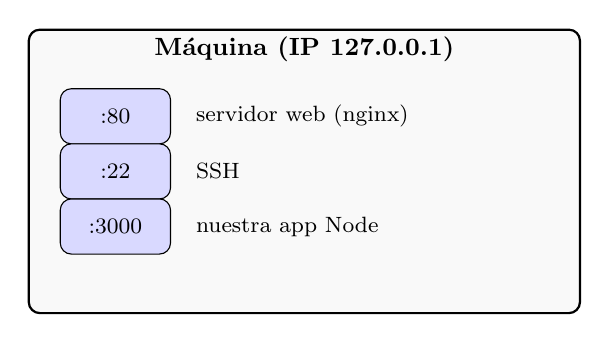
\begin{tikzpicture}[
        every node/.style={align=center, font=\small},
        machine/.style={rectangle, draw, thick, rounded corners, minimum width=7cm, minimum height=3.6cm, fill=gray!5},
        port/.style={rectangle, draw, rounded corners, minimum width=1.4cm, minimum height=0.7cm, fill=blue!15, font=\footnotesize},
        svc/.style={font=\footnotesize, anchor=west}
    ]
        \node[machine] (m) at (0, 0) {};
        \node[font=\bfseries\small] at (0, 1.55) {Máquina (IP 127.0.0.1)};

        \node[port] (p80)   at (-2.4,  0.7) {:80};
        \node[svc]          at (-1.5,  0.7) {servidor web (nginx)};

        \node[port] (p22)   at (-2.4,  0.0) {:22};
        \node[svc]          at (-1.5,  0.0) {SSH};

        \node[port] (p3000) at (-2.4, -0.7) {:3000};
        \node[svc]          at (-1.5, -0.7) {nuestra app Node};
    \end{tikzpicture}
    \end{center}

    \begin{block}{Puertos típicos}
        \begin{itemize}
            \item \textbf{80} $\rightarrow$ HTTP, \textbf{443} $\rightarrow$ HTTPS, \textbf{22} $\rightarrow$ SSH, \textbf{5432} $\rightarrow$ PostgreSQL.
            \item En desarrollo se suelen usar \textbf{3000}, \textbf{5000}, \textbf{8080} (no requieren permisos de root).
        \end{itemize}
    \end{block}
\end{frame}
